%%%%%%%%%%%%%%%%% CHAPTER 6 %%%%%%%%%%%%%%%%%%%%%%%%%%%%%%%%%
%%%%% Sorting %%%%%%%%%%%%%%%%%%%%%%%%%%%%%%%%%%%%%%%%%%%%%%%%
\section{Sorting}
Introduce need for sorting algorithms.  

Sorting is frequently necessary when data are being handled; for example in integration and differentiation the data are usually presented to the various algorithms in ascending or descending order (at least on the x-axis).

One may have tables of numbers, representing one or more explanatory variables, and one or more responses.   At times we may need to arrange these tables in an order dictated by one or another of these various variables.  
Alternatively we may want to find the median value or upper quartile of such a list -- this task requires sorting.  

When sorting, one can also carry along operations to maintain correspondence with other lists (for lack of better name lets call this sort-and-carry).

Tasks that fall under the broad category of sorting are:
\begin{itemize}
\item Sort ; rearrange an array of numbers into numerical order (ascending or descending).
\item Sort and carry along ; rearrange an array of numbers into numerical order while performing the same rearrangement of one or more additional arrays so that the correspondence between elements in all arrays is maintained (the sets of arrays are essentially a relational database -- so that each record (row) maintains the cross-record (fields; columns) relationship).
\item Index ; given an array, prepare an index table that is a table of pointers that indicates which number array element comes first in numerical order, which is second, and so on.
\item Rank ; given an array, prepare a rank table that tells the numerical rank of an array element.
\end{itemize}

The task of sorting $N$ elements requires on the order of $K \times N log_2 N$  operations.  The algorithm inventor tries to make $K$ as small as possible (understanding that $K=0$ is probably impossible).  
The three most useful sorting algorithms are:
\begin{enumerate}
\item Straight insertion sort;
\item Heapsort sort; and
\item Quicksort sort.
\end{enumerate}

The choice of method depends on the size of the list that needs to be sorted.  If the list is short (perhaps $N< 50$ elements) then straight insertion is fast enough, concise, and simple to program.     For a long list ($N > 1000$ elements) Quicksort is faster, but achieves the speed by use of extra memory.   Heapsort is also good for large lists, and is an in-place routine.

Python lists have a built-in \texttt{sort()} method that modifies the list \textbf{in-place} and a \texttt{sorted()} built-in function that builds a new sorted list from an iterable.  
So when sorting needs to be done, you would  use the built-in tools.  However, because it is a useful programming construct, the three sorting algorithms are presented as primitive code.


\subsection{Straight Insertion}
The straight insertion sort is the algorithm a card player would use to sort cards.  
Pick out the second card and put it into order with respect to the first; then pick the third card and insert it into sequence with the first two; continue until the last card is picked out and inserted.   
Once the last card is sequenced, the result is a sorted deck (list). Figure \ref{fig:StraightInsertionSort} is a Python implementation of such an algorithm.   
\begin{figure}[h!] %  figure placement: here, top, bottom, or page
   \centering
   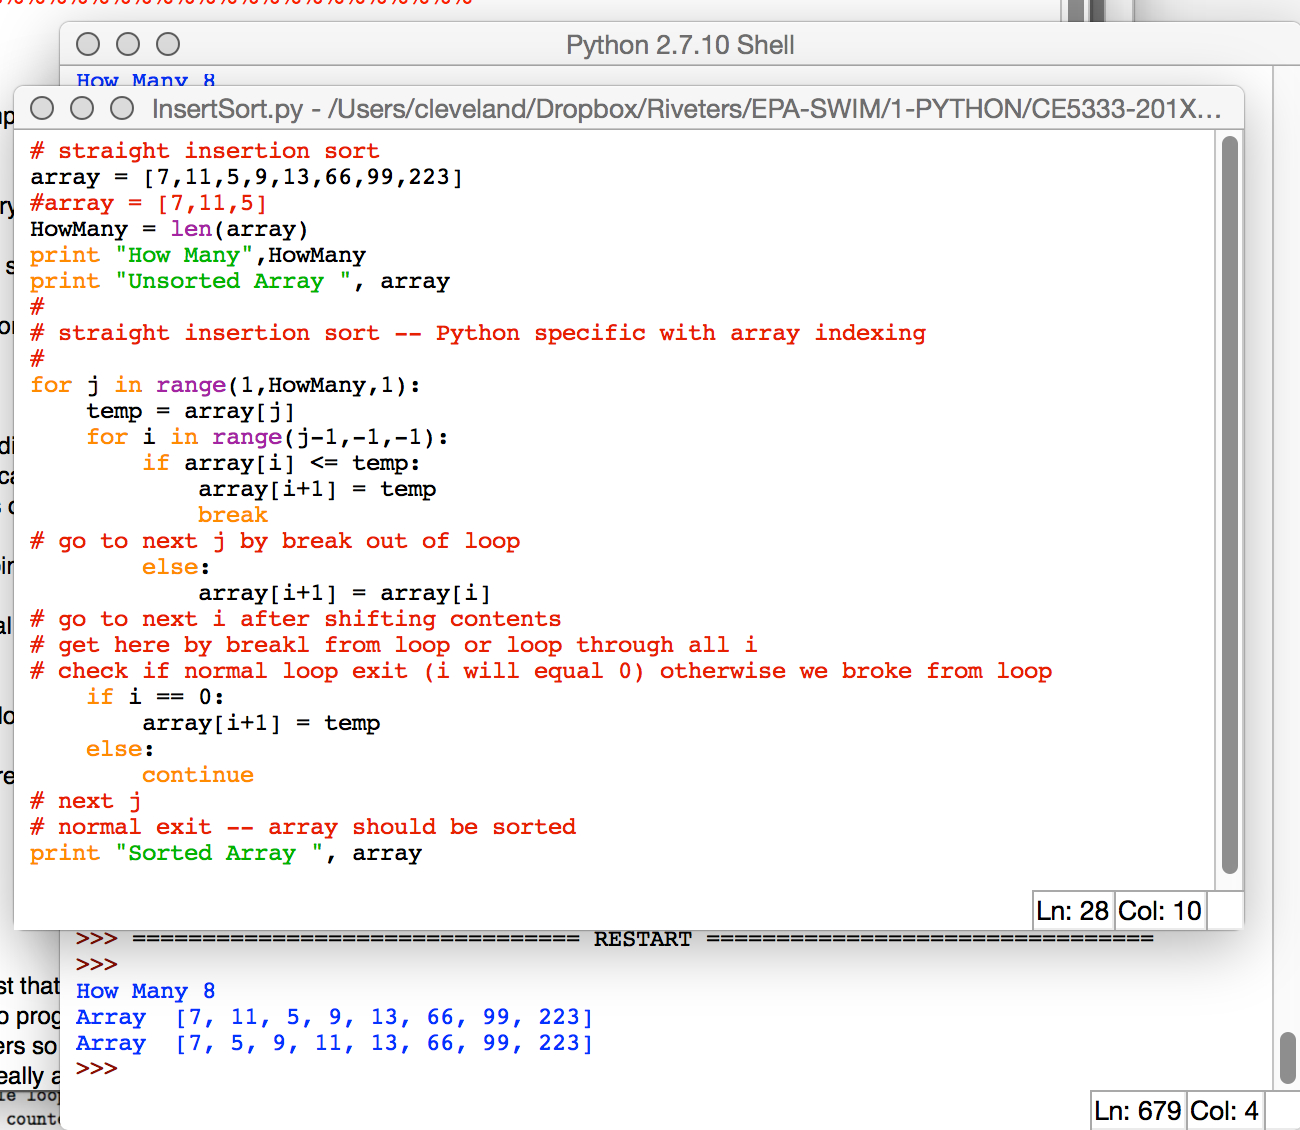
\includegraphics[width=5in]{./6-Sorting/StraightInsertionSort.jpg} 
   \caption{Example of Straight-Insertion Sort in Python.  Keep in mind this code is meant for small arrays $N<50$.}
   \label{fig:StraightInsertionSort}
\end{figure}
\clearpage
\subsubsection{Sort-and-Carry} 
Describe the algorithm.  Include pseudo code.
Provide python example of sort
Provide python example of sort-and-carry 
%%%%%%
\subsection{Heapsort sort}
Describe the algorithm.  Include pseudo code.
Provide python example of sort
Provide python example of sort-and-carry 
\subsection{Quicksort sort}
Describe the algorithm.  Include pseudo code.
Provide python example of sort
Provide python example of sort-and-carry 
\subsection{Related concepts}
\subsection{Exercise}

%%%%%%%%%%%%%%%%%%%%%%%%%%%%%%%%%%%%%%%%%%%%%%%%%%%%%%